\documentclass[twoside,11pt,a4paper]{article}

\usepackage[utf8]{inputenc}
\usepackage{amsmath, amssymb, latexsym}
\DeclareMathOperator{\ReLU}{ReLU}
\newcommand{\KL}{\ensuremath{\mathrm{KL}}}
\newcommand{\Ber}{\ensuremath{\mathrm{Ber}}}

\usepackage{tikz}
\usepackage{xcolor}
\definecolor{fc}{HTML}{1E90FF}
\definecolor{h}{HTML}{228B22}
\definecolor{bias}{HTML}{87CEFA}
\definecolor{noise}{HTML}{8B008B}
\definecolor{conv}{HTML}{FFA500}
\definecolor{pool}{HTML}{B22222}
\definecolor{up}{HTML}{B22222}
\definecolor{view}{HTML}{FFFFFF}
\definecolor{bn}{HTML}{FFD700}
\tikzset{fc/.style={black,draw=black,fill=fc,rectangle,minimum height=1cm}}
\tikzset{h/.style={black,draw=black,fill=h,rectangle,minimum height=1cm}}
\tikzset{bias/.style={black,draw=black,fill=bias,rectangle,minimum height=1cm}}
\tikzset{noise/.style={black,draw=black,fill=noise,rectangle,minimum height=1cm}}
\tikzset{conv/.style={black,draw=black,fill=conv,rectangle,minimum height=1cm}}
\tikzset{pool/.style={black,draw=black,fill=pool,rectangle,minimum height=1cm}}
\tikzset{up/.style={black,draw=black,fill=up,rectangle,minimum height=1cm}}
\tikzset{view/.style={black,draw=black,fill=view,rectangle,minimum height=1cm}}
\tikzset{bn/.style={black,draw=black,fill=bn,rectangle,minimum height=1cm}}

\usepackage{xspace}
\newcommand*{\eg}{\emph{e.g.}\@\xspace}
\newcommand*{\Eg}{\emph{E.g.}\@\xspace}
\newcommand*{\ie}{\emph{i.e.}\@\xspace}
\newcommand*{\etc}{\emph{etc.}\@\xspace}
\newcommand*{\etal}{\emph{et al.}\@\xspace}
\newcommand*{\cf}{\emph{cf.}\@\xspace}
\newcommand*{\vs}{\emph{vs.}\@\xspace}

\begin{document}

\begin{figure}
  \centering
  \hspace*{-0.75cm}
  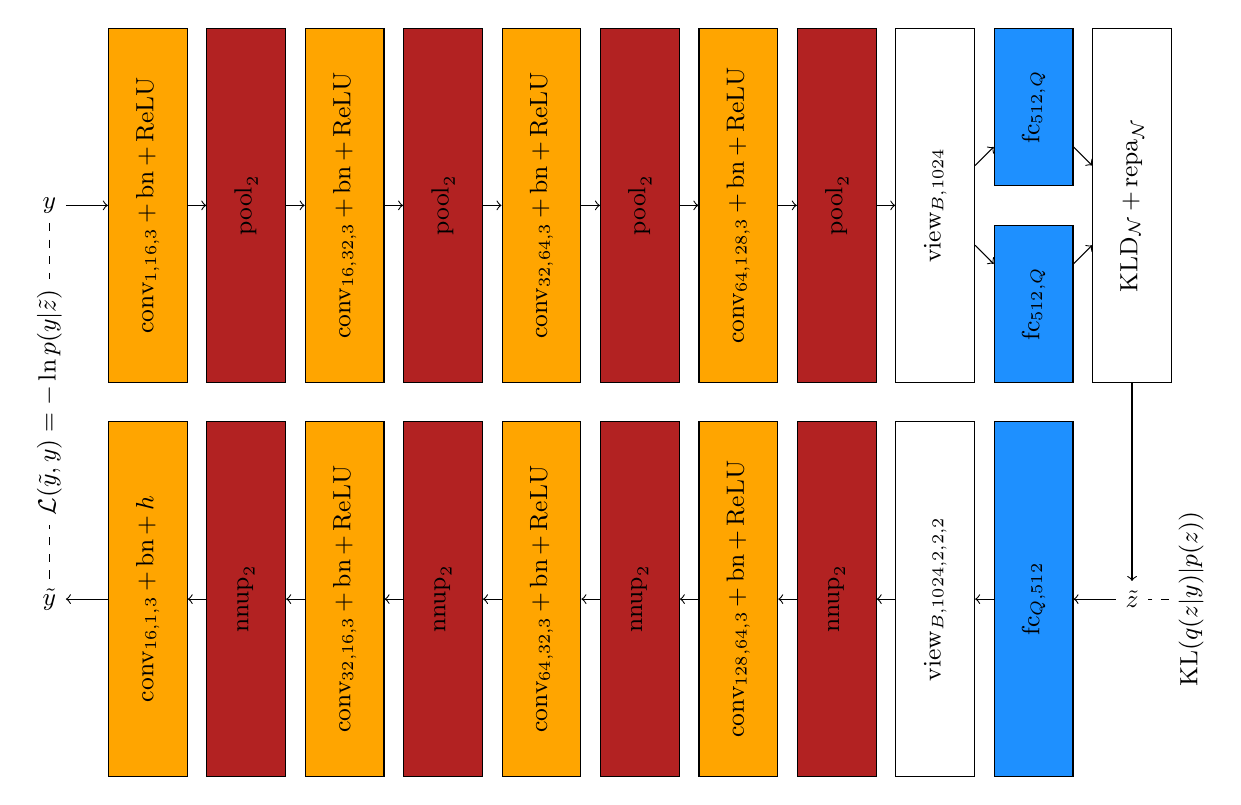
\begin{tikzpicture}
    \node (y) at (0,0) {\small$y$};

    \node[conv,rotate=90,minimum width=4.5cm] (conv1) at (1.25,0) {\small$\text{conv}_{1, 16, 3}$\,+\,$\text{bn}$\,+\,$\ReLU$};
    \node[pool,rotate=90,minimum width=4.5cm] (pool1) at (2.5,0) {\small$\text{pool}_{2}$};
    \node[conv,rotate=90,minimum width=4.5cm] (conv2) at (3.75,0) {\small$\text{conv}_{16, 32, 3}$\,+\,$\text{bn}$\,+\,$\ReLU$};
    \node[pool,rotate=90,minimum width=4.5cm] (pool2) at (5,0) {\small$\text{pool}_{2}$};
    \node[conv,rotate=90,minimum width=4.5cm] (conv3) at (6.25,0) {\small$\text{conv}_{32, 64, 3}$\,+\,$\text{bn}$\,+\,$\ReLU$};
    \node[pool,rotate=90,minimum width=4.5cm] (pool3) at (7.5,0) {\small$\text{pool}_{2}$};
    \node[conv,rotate=90,minimum width=4.5cm] (conv4) at (8.75,0) {\small$\text{conv}_{64, 128, 3}$\,+\,$\text{bn}$\,+\,$\ReLU$};
    \node[pool,rotate=90,minimum width=4.5cm] (pool4) at (10,0) {\small$\text{pool}_{2}$};
    
    \node[view,rotate=90,minimum width=4.5cm] (view4) at (11.25,0) {\small$\text{view}_{B, 1024}$};
    
    \node[fc,rotate=90, minimum width = 2cm] (fc51) at (12.5,1.25) {\small$\text{fc}_{512, Q}$};
    \node[fc,rotate=90, minimum width = 2cm] (fc52) at (12.5,-1.25) {\small$\text{fc}_{512, Q}$};
  
    \node[view,rotate=90,minimum width=4.5cm] (kld) at (13.75,0) {\small$\text{KLD}_{\mathcal{N}}$\,+\,$\text{repa}_{\mathcal{N}}$};
    
    \node (z) at (13.75,-5){\small$\tilde{z}$};
    
    \node[fc,rotate=90,minimum width=4.5cm] (fc6) at (12.5,-5) {\small$\text{fc}_{Q, 512}$};
    \node[view,rotate=90,minimum width=4.5cm] (view6) at (11.25,-5) {\small$\text{view}_{B, 1024, 2, 2, 2}$};
    
    \node[up,rotate=90,minimum width=4.5cm] (up7) at (10,-5) {\small$\text{nnup}_{2}$};
    \node[conv,rotate=90,minimum width=4.5cm] (conv7) at (8.75,-5) {\small$\text{conv}_{128, 64, 3}$\,+\,$\text{bn}$\,+\,$\ReLU$};
    \node[up,rotate=90,minimum width=4.5cm] (up8) at (7.5,-5) {\small$\text{nnup}_{2}$};
    \node[conv,rotate=90,minimum width=4.5cm] (conv8) at (6.25,-5) {\small$\text{conv}_{64, 32, 3}$\,+\,$\text{bn}$\,+\,$\ReLU$};
    \node[up,rotate=90,minimum width=4.5cm] (up9) at (5,-5) {\small$\text{nnup}_{2}$};
    \node[conv,rotate=90,minimum width=4.5cm] (conv9) at (3.75,-5) {\small$\text{conv}_{32, 16, 3}$\,+\,$\text{bn}$\,+\,$\ReLU$};
    \node[up,rotate=90,minimum width=4.5cm] (up10) at (2.5,-5) {\small$\text{nnup}_{2}$};
    \node[conv,rotate=90,minimum width=4.5cm] (conv10) at (1.25,-5) {\small$\text{conv}_{16, 1, 3}$\,+\,$\text{bn}$\,+\,$h$};
    
    \node (ry) at (0,-5) {\small$\tilde{y}$};
    
    \draw[->] (y) -- (conv1);
    \draw[->] (conv1) -- (pool1);
    \draw[->] (pool1) -- (conv2);
    
    \draw[->] (conv2) -- (pool2);
    \draw[->] (pool2) -- (conv3);
    
    \draw[->] (conv3) -- (pool3);
    \draw[->] (pool3) -- (conv4);
    
    \draw[->] (conv4) -- (pool4);
    \draw[->] (pool4) -- (view4);
    
    \draw[->] (view4) -- (fc51);
    \draw[->] (view4) -- (fc52);
    
    \draw[->] (fc51) -- (kld);
    \draw[->] (fc52) -- (kld);
    
    \draw[->] (kld) -- (z);
    \draw[->] (z) -- (fc6);
    \draw[->] (fc6) -- (view6);
    
    \draw[->] (view6) -- (up7);
    \draw[->] (up7) -- (conv7);
    
    \draw[->] (conv7) -- (up8);
    \draw[->] (up8) -- (conv8);
    
    \draw[->] (conv8) -- (up9);
    \draw[->] (up9) -- (conv9);
    
    \draw[->] (conv9) -- (up10);
    \draw[->] (up10) -- (conv10);
    
    \draw[->] (conv10) -- (ry);

    \node[rotate=90] (L) at (0, -2.5) {\small$\mathcal{L}(\tilde{y}, y) = -\ln p(y | \tilde{z})$};
    \draw[-,dashed] (y) -- (L);
    \draw[-,dashed] (ry) -- (L);

    \node[rotate=90] (KLD) at (14.5, -5) {\small$\KL(q(z|y) | p(z))$};
    \draw[-,dashed] (KLD) -- (z);
  \end{tikzpicture}
  \vskip 6px
  \caption{An illustration of a Gaussian variational auto-encoder with
  four convolutional stages in both encoder and decoder. This is also the
  architecture used in experiments in Chapter \ref{ch:experiments} where
  we assume volumes of size
  $32 \times 32 \times 32$ such that the spatial size just before
  the fully connected layers of the encoder is $2 \times 2 \times 2$
  resulting in a $1024$-dimensional representation when considering $128$
  channels.}
  \label{subfig:experiments-2d-architecture-vae}
\end{figure}

\begin{figure}
  \centering
  \hspace*{-0.75cm}
  \begin{tikzpicture}
    \node (x) at (0,0) {\small$x$};

    \node[conv,rotate=90,minimum width=4.5cm] (conv1) at (2.5,0) {\small$\text{conv}_{1, 16, 3}$\,+\,$\text{bn}$\,+\,$\ReLU$};
    \node[pool,rotate=90,minimum width=4.5cm] (pool1) at (3.75,0) {\small$\text{pool}_{2}$};
    \node[conv,rotate=90,minimum width=4.5cm] (conv2) at (5,0) {\small$\text{conv}_{16, 32, 3}$\,+\,$\text{bn}$\,+\,$\ReLU$};
    \node[pool,rotate=90,minimum width=4.5cm] (pool2) at (6.25,0) {\small$\text{pool}_{2}$};
    \node[conv,rotate=90,minimum width=4.5cm] (conv3) at (7.5,0) {\small$\text{conv}_{32, 64, 3}$\,+\,$\text{bn}$\,+\,$\ReLU$};
    \node[pool,rotate=90,minimum width=4.5cm] (pool3) at (8.75,0) {\small$\text{pool}_{2}$};
    \node[conv,rotate=90,minimum width=4.5cm] (conv4) at (10,0) {\small$\text{conv}_{64, 128, 3}$\,+\,$\text{bn}$\,+\,$\ReLU$};
    \node[pool,rotate=90,minimum width=4.5cm] (pool4) at (11.25,0) {\small$\text{pool}_{2}$};
    
    \node[view,rotate=90,minimum width=4.5cm] (view4) at (12.5,0) {\small$\text{view}_{B, 1024}$};
    
    \node[fc,rotate=90, minimum width = 2cm] (fc51) at (13.75,1.25) {\small$\text{fc}_{512, Q}$};
    \node[fc,rotate=90, minimum width = 2cm] (fc52) at (13.75,-1.25) {\small$\text{fc}_{512, Q}$};
  
    \node[view,rotate=90,minimum width=4.5cm] (kld) at (15,0) {\small$\text{KLD}_{\mathcal{N}}$\,+\,$\text{repa}_{\mathcal{N}}$};
    
    \node (z) at (15,-5){\small$\tilde{z}$};
    
    \node[fc,rotate=90,minimum width=4.5cm] (fc6) at (13.75,-5) {\small$\text{fc}_{Q, 512}$};
    \node[view,rotate=90,minimum width=4.5cm] (view6) at (12.5,-5) {\small$\text{view}_{B, 1024, 2, 2, 2}$};
    
    \node[up,rotate=90,minimum width=4.5cm] (up7) at (11.25,-5) {\small$\text{nnup}_{2}$};
    \node[conv,rotate=90,minimum width=4.5cm] (conv7) at (10,-5) {\small$\text{conv}_{128, 64, 3}$\,+\,$\text{bn}$\,+\,$\ReLU$};
    \node[up,rotate=90,minimum width=4.5cm] (up8) at (8.75,-5) {\small$\text{nnup}_{2}$};
    \node[conv,rotate=90,minimum width=4.5cm] (conv8) at (7.5,-5) {\small$\text{conv}_{64, 32, 3}$\,+\,$\text{bn}$\,+\,$\ReLU$};
    \node[up,rotate=90,minimum width=4.5cm] (up9) at (6.25,-5) {\small$\text{nnup}_{2}$};
    \node[conv,rotate=90,minimum width=4.5cm] (conv9) at (5,-5) {\small$\text{conv}_{32, 16, 3}$\,+\,$\text{bn}$\,+\,$\ReLU$};
    \node[up,rotate=90,minimum width=4.5cm] (up10) at (3.75,-5) {\small$\text{nnup}_{2}$};
    \node[conv,rotate=90,minimum width=4.5cm] (conv10) at (2.5,-5) {\small$\text{conv}_{16, 1, 3}$\,+\,$\text{bn}$\,+\,$h$};
    
    \node[view,rotate=90,minimum width=4.5cm] (kld2) at (1.25,-5) {\small$\text{KLD}_{\Ber}$\,+\,$\text{repa}_{\Ber}$\,+\,$\sigma$};
    \node (ry) at (0,-5) {\small$\tilde{y}$};
    
    \node[conv,rotate=90,minimum width=4.5cm] (conv11) at (1.25,-10) {\small$\text{conv}_{1, 16, 3}$\,+\,$\text{bn}$\,+\,$\ReLU$};
    \node[conv,rotate=90,minimum width=4.5cm] (conv12) at (2.5,-10) {\small$\text{conv}_{16, 32, 3}$\,+\,$\text{bn}$ + $\ReLU$};
    \node[conv,rotate=90,minimum width=4.5cm] (conv13) at (3.75,-10) {\small$\text{conv}_{32, 64, 3}$\,+\,$\text{bn}$\,+\,$\ReLU$};
    \node[conv,rotate=90,minimum width=4.5cm] (conv14) at (5,-10) {\small$\text{conv}_{64, 128, 3}$\,+\,$\text{bn}$\,+\,$\ReLU$};
    \node[conv,rotate=90,minimum width=4.5cm] (conv15) at (6.25,-10) {\small$\text{conv}_{128, 64, 3}$\,+\,$\text{bn}$\,+\,$\ReLU$};
    \node[conv,rotate=90,minimum width=4.5cm] (conv16) at (7.5,-10) {\small$\text{conv}_{64, 32, 3}$\,+\,$\text{bn}$\,+\,$\ReLU$};
    \node[conv,rotate=90,minimum width=4.5cm] (conv17) at (8.74,-10) {\small$\text{conv}_{32, 16, 3}$\,+\,$\text{bn}$\,+\,$\ReLU$};
    \node[conv,rotate=90,minimum width=4.5cm] (conv18) at (10,-10) {\small$\text{conv}_{16, 1, 3}$\,+\,$\text{bn}$\,+\,$\sigma$};
    
    \node (rx) at (15, -10) {\small$\tilde{x}$};
    
    \draw[->] (y) -- (conv1);
    \draw[->] (conv1) -- (pool1);
    \draw[->] (pool1) -- (conv2);
    
    \draw[->] (conv2) -- (pool2);
    \draw[->] (pool2) -- (conv3);
    
    \draw[->] (conv3) -- (pool3);
    \draw[->] (pool3) -- (conv4);
    
    \draw[->] (conv4) -- (pool4);
    \draw[->] (pool4) -- (view4);
    
    \draw[->] (view4) -- (fc51);
    \draw[->] (view4) -- (fc52);
    
    \draw[->] (fc51) -- (kld);
    \draw[->] (fc52) -- (kld);
    
    \draw[->] (kld) -- (z);
    \draw[->] (z) -- (fc6);
    \draw[->] (fc6) -- (view6);
    
    \draw[->] (view6) -- (up7);
    \draw[->] (up7) -- (conv7);
    
    \draw[->] (conv7) -- (up8);
    \draw[->] (up8) -- (conv8);
    
    \draw[->] (conv8) -- (up9);
    \draw[->] (up9) -- (conv9);
    
    \draw[->] (conv9) -- (up10);
    \draw[->] (up10) -- (conv10);
    
    \draw[->] (conv10) -- (kld2);
    \draw[->] (kld2) -- (ry);
    \draw[-] (ry) -- (0, -10);
    \draw[->] (0, -10) -- (conv11);
    
    \draw[->] (conv11) -- (conv12);
    \draw[->] (conv12) -- (conv13);
    
    \draw[->] (conv13) -- (conv14);
    \draw[->] (conv14) -- (conv15);
    
    \draw[->] (conv15) -- (conv16);
    \draw[->] (conv16) -- (conv17);
    
    \draw[->] (conv17) -- (conv18);
    \draw[->] (conv18) -- (rx);

    \node[rotate=90] (L2) at (15, -11.5) {\small$\mathcal{L}(\tilde{x}, x)$};
    \draw[-,dashed] (rx) -- (L2);

    \node[rotate=90] (L1) at (0, 1.5) {\small$\mathcal{L}(\tilde{x}, x)$};
    \draw[-,dashed] (x) -- (L1);

    \node[rotate=90] (KLD2) at (0, -2.5) {\small$\KL(p(y|x)|p(y|z))$};
    \draw[-,dashed] (ry) -- (KLD2);

    \node[rotate=90] (KLD1) at (15, -7.5) {\small$\KL(q(z|y)|p(z))$};
    \draw[-,dashed] (z) -- (KLD1);
  \end{tikzpicture}
  \vskip 6px
  \caption{Illustration of the extended variational auto-encoder as
  also.
  It is worth comparing the illustrated implementation with Figure
  \ref{subfig:experiments-2d-architecture-vae} to understand that the
  generative model $p(y | z)$ are taken from the shape prior and the new
  recognition model $q(z | x)$ follows the architecture of $q(y| z)$. 
  In particular, the decoder, \ie $p(y|z)$, is kept fixed after learning the shape prior.
  The only completely new part is the convolutional neural network implementing the
  observation model $p(x|y)$. It consists of
  of eight convolutional stages including batch normalization and non-linearity.
  Here, no pooling layers can be found as the size of the output $x$
  matches the size of its input $y$. We additionally make the loss $\mathcal{L}(\tilde{x}, x)$
  between reconstructed observation $\tilde{x}$ and original observation $x$
  as well as the Kullback-Leibler divergences $\KL(q(z|y)|p(z))$, for the prior $p(z)$,
  and $\KL(p(y|x)|p(y|z))$, tying observations to predicted shapes, explicit.}
  \label{fig:shape-inference-evae}
\end{figure}

\end{document}